%!TEX program = xelatex
% not lualatex because of a pgf bug: https://sourceforge.net/p/pgf/bugs/384/
\PassOptionsToPackage{table,svgnames}{xcolor}
\documentclass[11pt, book, english, french]{upmethodology-document}
%!TEX root = ./RAPPORT_A17_INFO_ST40_PINARD_MAXIME.tex

% Encoding
	%\usepackage[utf8]{inputenc}
	%\usepackage[latin1]{inputenc}
	\usepackage[T1]{fontenc}

% Language
	%\usepackage[francais,english]{babel} % Second language = main language
	\usepackage[french]{translator}

% Show a summary of the layout of the current document with \layout.
	%\usepackage{layout}

% For easy management of document margins and the document page size.
	%\usepackage[top=2cm, bottom=1.8cm, left=1.8cm, right=1.8cm, head=14pt, foot=36pt]{geometry}

% Lets you change line spacing.
	%\usepackage{setspace}

% Euro symbol
	%\usepackage{eurosym}

% Fonts (include only one)
	%\usepackage{bookman}
	%\usepackage{charter}
	%\usepackage{newcent}
	\usepackage{lmodern}
	%\usepackage{mathpazo}
	%\usepackage{mathptmx}

% Enables typesetting of hyperlinks
	%\usepackage{url}
	\usepackage{hyperref}

% Verbatim environment
	%\usepackage{verbatim}
	%\usepackage{moreverb}
	\usepackage{fancyvrb}

% Code listing
	\usepackage{listings}

% To change header and footer of any page of the document.
	%\usepackage{fancyhdr}

% Allows you to insert graphic files within a document.
	%\usepackage{graphicx}

% Allows figures or tables to have text wrapped around them.
	%\usepackage{wrapfig}

% Adds support for colored text.
	\usepackage{xcolor}

% Allows tables rows and columns to be colored, and even individual cells.
	%\usepackage{colortbl}

% Mathematics
	\usepackage{amsmath}
	\usepackage{amssymb}
	\usepackage{mathrsfs}
	%\usepackage{asmthm}
	%\usepackage{mathtools}
	%\usepackage{bm} % Greek letters in math mode

% Provide the array and tabular environments
	\usepackage{array}

% Provide the tabularx environment
	\usepackage{tabularx}

% Provide the multirow command
	\usepackage{multirow}

% Provides control over the layout of the three basic list environments: enumerate, itemize and description.
	%\usepackage{enumitem}

% Interface to sectioning commands for selection from various title styles
	%\usepackage[nobottomtitles]{titlesec}

% Highly customized stacking of objects, insets, baseline changes, etc.
	\usepackage{stackengine}

% Routines for constrained scaling and stretching of objects, relative to a reference object or in absolute terms
	\usepackage{scalerel}

% Provides control over the typography of the Table of Contents, List of Figures and List of Tables, and the ability to create new ‘List of ...’.
	%\usepackage{tocloft}
	%\usepackage{titletoc}

% Advanced bibliography handling.
	%\usepackage{bibtex}
	%\usepackage{biblatex}

% Allows customization of appearance and placement of captions for figures, tables, etc.
	\usepackage[justification=centering]{caption}

% Provides the multicols environment which typesets text into multiple columns.
	%\usepackage{multicol}

% This package simplifies the insertion of external multi-page PDF or PS documents.
	%\usepackage{pdfpages}

% Prints out all index entries in the left margin of the text.
	%\usepackage{showidx}

% Allow to define multiple floats (figures, tables) within one environment giving individual captions and labels in the form 1a, 1b.
	%\usepackage{subcaption}

% Lets you insert notes of stuff to do with the syntax \todo{Add details.}.
	%\usepackage{todonotes}

% Text Companion fonts, which provide many text symbols (such as baht, bullet, copyright, musicalnote, onequarter, section, and yen), in the TS1 encoding.
	%\usepackage{textcomp}

% Supply landscape environment
	\usepackage{pdflscape}

% Floating elements placement
	\usepackage{float}

% Add document elements like a bibliography or an index to the Table of Contents.
	\usepackage[notindex,nottoc,notlot,notlof]{tocbibind}

% Allow TeX pictures or other TeX code to be compiled standalone or as part of a main document
	%\usepackage[subpreambles=true]{standalone}
	\usepackage{standalone}
	\usepackage{import}

% PGF-TikZ
	\usepackage{pgf}
	\usepackage{tikz}
	\usepackage{pgf-umlsd}
	\usepackage{pgfgantt}

% Change the typesetting of footnotes
	\usepackage[perpage,bottom]{footmisc}

% Defines commands \counterwithin and \counterwithout
	\usepackage{chngcntr}

% Allow creation of glossaries
	\usepackage[acronym,toc]{glossaries}

% Personnal packages
	\usepackage{packages/MagicListings}

%!TEX root = ./RAPPORT_A17_INFO_ST40_PINARD_MAXIME.tex

%----------------------------------------
% Figures configuration
%----------------------------------------

\usetikzlibrary{shapes}
\usetikzlibrary{arrows.meta}
\usetikzlibrary{calc}

\definecolor{bg_color}{RGB}{250,250,229}

\colorlet{color1}{cyan!50}
\colorlet{color2}{red!30!green!40}
\colorlet{color3}{orange!50}
\colorlet{color4}{violet!60!blue!55}

\newganttlinktype{bartobardown}{
	\ganttsetstartanchor{south east}
	\ganttsetendanchor{north west}
	\draw [/pgfgantt/link] (\xLeft, \yUpper) -- (\xRight, \yLower);
}
\newganttlinktype{bartobarup}{
	\ganttsetstartanchor{north east}
	\ganttsetendanchor{south west}
	\draw [/pgfgantt/link] (\xLeft, \yUpper) -- (\xRight, \yLower);
}
\newganttlinktype{milestonetobardown}{
	\ganttsetstartanchor{south}
	\ganttsetendanchor{north west}
	\draw [/pgfgantt/link] (\xLeft, \yUpper) -- (\xRight, \yLower);
}
\newganttlinktype{bartomilestonedown}{
	\ganttsetstartanchor{south east}
	\ganttsetendanchor{north}
	\draw [/pgfgantt/link] (\xLeft, \yUpper) -- (\xRight, \yLower);
}


%----------------------------------------
% upmethodology commands redefinition
%----------------------------------------

\makeatletter

% Remove 'Initials' column from validators
\renewcommand{\upm@document@addvalidator}[3][]{%
	\global\protected@edef\thevalidatorlist{\thevalidatorlist\protect\Ifnotempty{\thevalidatorlist}{,} \protect\upmmakename{#2}{#3}{~}}

	\global\protected@edef\upm@document@validator@tab@commented{\upm@document@validator@tab@commented \protect\upmmakename{#2}{#3}{~} & 
	& \protect\Ifnotempty{#1}{\protect\href{mailto:#1}{#1}}\\}

	\ifupm@document@validator@tab@hascomment\else
		\global\protected@edef\upm@document@validator@tab{\upm@document@validator@tab \protect\upmmakename{#2}{#3}{~} & 
		\protect\Ifnotempty{#1}{\protect\href{mailto:#1}{#1}}\\}
	\fi
}
\renewcommand{\upm@document@addvalidatorstar}[4][]{%
	\global\protected@edef\thevalidatorlist{\thevalidatorlist\protect\Ifnotempty{\thevalidatorlist}{,} \protect\upmmakename{#2}{#3}{~}}

	\global\let\upm@document@validator@tab\relax

	\global\protected@edef\upm@document@validator@tab@commented{\upm@document@validator@tab@commented \protect\upmmakename{#2}{#3}{~} & 
	#4 & \protect\Ifnotempty{#1}{\protect\href{mailto:#1}{#1}}\\}

	\upm@document@validator@tab@hascommenttrue
}
\renewcommand{\upmdocumentvalidators}[1][\linewidth]{%
	\ifupm@document@validator@tab@hascomment%
		\Ifnotempty{\upm@document@validator@tab@commented}{%
		\noindent\expandafter\begin{mtabular}[#1]{3}{|X|l|c|}%
		\tabulartitle{\upm@lang@document@validators}%
		\tabularheader{\upm@lang@document@names}{\upm@lang@document@comments}{\upm@lang@document@emails}%
		\upm@document@validator@tab@commented
		\hline%
		\expandafter\end{mtabular}\par\vspace{.5cm}}%
	\else%
		\Ifnotempty{\upm@document@validator@tab}{%
		\noindent\expandafter\begin{mtabular}[#1]{2}{|X|c|}%
		\tabulartitle{\upm@lang@document@validators}%
		\tabularheader{\upm@lang@document@names}{\upm@lang@document@emails}%
		\upm@document@validator@tab
		\hline%
		\expandafter\end{mtabular}\par\vspace{.5cm}}%
	\fi%
}

% Remove history from document info page
\renewcommand{\upmdocinfopage}{
	\thispagestyle{plain}
	\upmdocumentsummary\upmdocumentauthors\upmdocumentvalidators\upmdocumentinformedpeople\clearpage%
}

% Decrease space after upmcaution upminfo and upmquestion message boxes
\renewenvironment{upm@highligh@box}[2]{%
	\par
	\vspace{.5cm}
	\begin{tabular}{|p{#1}|}
	\hline
	\begin{window}[0,l,{\mbox{\includegraphics[width=1cm]{#2}}},{}]
}{%
	\end{window}\\ \hline \end{tabular}
	%\vspace{.5cm}
	\par
}

\makeatother

%----------------------------------------
% upmethodology informations
%----------------------------------------

% Document Information and Declaration
\declaredocument{Rapport de stage ST40 - A2017}{Développement et fiabilisation d’un module de désassemblage interne}{-}

% Document Authors
\addauthor*[maxime.pinard@utbm.fr]{Maxime}{Pinard}{Étudiant en branche INFO}

% Document Validators
\addvalidator*[jean-charles.creput@utbm.fr]{Jean-Charles}{Creput}{Suiveur UTBM}
\addvalidator*[benoit.amiaux@intradef.gouv.fr]{Benoît}{Amiaux}{Tuteur en entreprise}

% Informed People
\addinformed*[jean-charles.creput@utbm.fr]{Jean-Charles}{Creput}{Suiveur UTBM}
\addinformed*[benoit.amiaux@intradef.gouv.fr]{Benoît}{Amiaux}{Tuteur en entreprise}
\addinformed*[laure.foissard@intradef.gouv.fr]{Laure}{Foissard}{Responsable administratif (DRH)}

% Copyright and Publication Information
\setcopyrighter{Maxime Pinard}
\setpublisher{l'Universitée de Technologie de Belfort Montbéliard}

% Version
\incversion{\makedate{\the\day}{\the\month}{\the\year}}{Version initiale.}{\upmpublic}

%----------------------------------------
% utbmcovers informations
%----------------------------------------

\UseExtension{utbmcovers}

\setutbmfrontillustration{cover}
\setutbmtitle{Développement et fiabilisation d’un module de désassemblage interne}
\setutbmsubtitle{Rapport de stage ST40 - A2017}
\setutbmstudent{Maxime Pinard}
\setutbmstudentdepartment{Département Informatique}
\setutbmstudentpathway{}
\setutbmcompany{Direction générale de l'armement\\Maîtrise de l’information}
\setutbmcompanyaddress{Route de Laillé\\ 35131 Bruz, France}
\setutbmcompanywebsite{\href{http://www.defense.gouv.fr/dga}{\color{utbm_cover_main_shadow_text}{http://www.defense.gouv.fr/dga}}}
\setutbmcompanytutor{Benoît Amiaux}
\setutbmschooltutor{Jean-Charles Creput}
\setutbmkeywords{
	% Branche d'activité économique
	Armement \textendash{}
	SSII, services informatiques \textendash{}
	% Métiers
	Informatique \textendash{}
	Etude, développement \textendash{}
	% Domaine technologique
	Génie logiciel \textendash{}
	Sécurité \textendash{}
	% Application physique directe
	Logiciel d'analyse de données \textendash{}
	Analyse de binaires
}
\setutbmabstract{
	La Direction Générale de l'Armement (DGA) est une direction du Ministère des Armées qui a de nombreuses missions dont celle de préparer l'avenir des systèmes de défense français, pour cela plusieurs centres d'expertise et d'essais sont répartis en France tels que la DGA Maîtrise de l'Information (DGA MI) situé près de Rennes. La DGA MI a pour mission des études, expertises et essais dans les domaines de la guerre électronique, des systèmes d'armes, des systèmes d'information, des télécommunications, de la sécurité de l'information et des composants électroniques.
	\vspace{12pt}\\
	Au sein de la DGA MI des équipes travaillent sur l’analyse de binaires dont le code source est inconnu, pour cela deux types d'analyses sont utilisées, l'analyse dynamique en suivant l'exécution du programme à l'aide d'un débogueur et l'analyse statique en étudiant le code désassemblé sans exécuter le programme.
	\vspace{12pt}\\
	GenDbg est un débogueur générique développé en interne de la DGA MI, conçu pour pouvoir déboguer tout type de programme, il repose sur de nombreux modules spécifiques aux caractéristiques du programme débogué. Le module de désassemblage pour les architectures de processeurs MIPS de GenDbg étant obsolète et non maintenu, ma première mission a été de réaliser une nouvelle implémentation de ce dernier en utilisant la librairie de désassemblage Capstone.
	\vspace{12pt}\\
	Hex-Rays IDA est un logiciel d'analyse statique qui permet de documenter un binaire pour en comprendre le fonctionnement, la DGA MI développe et maintient un plugin IDA nommé YaCo qui permet de travailler à plusieurs sur une même base de code. YaCo, initialement codé en Python, a été porté en C++, la deuxième mission de mon stage a été de réaliser le portage C++ et l'amélioration des parties responsables de la gestion du dépôt Git et des événements IDA.
}

%----------------------------------------
% Listings
%----------------------------------------

\lstalias[gendbg]{C}[GenDbg]{C}
\lstdefinelanguage[gendbg]{C}{
	language={[StandardLibrary]C},
	morekeywords=[1]{
		__cdecl
	},
	morekeywords=[2]{
		DWORD
	},
	morekeywords=[2]{
		AsmBankInfo_T,
		AsmAddressSpaceInfo_T,
		AsmAddressTypeInfo_T,
		AsmGroupRegisterInfo_T,
		AsmDataInfo_T,
		AsmDecodedInstruction_T,
		AsmInstructionInfo_T,
		AsmModuleInfo_T,
		CPUCtx_T,
		GenDbgHelperAsmInfo_T,
		MemoryAddress_T,
		MemoryArea_T,
		ViewCtx_T,
		AsmModuleFnIdx_T,
		MIPS_RegisterId_T
	},
	morekeywords=[2]{
		cs_insn,
		cs_detail,
		cs_x86,
		cs_arm64,
		cs_arm,
		cs_m68k,
		cs_mips,
		cs_ppc,
		cs_sparc,
		cs_sysz,
		cs_xcore,
		cs_tms320c64x,
		cs_mips_op,
		mips_reg,
		mips_op_mem
	},
	morekeywords=[3]{
		CS_MNEMONIC_SIZE
	}
}

\lstalias[yaco]{C}[YaCo]{C}
\lstdefinelanguage[yaco]{C}{
	language={[StandardLibrary]C},
	morekeywords=[1]{
		__cdecl
	},
	morekeywords=[2]{
		ssize_t,
		hook_type_t,
		hook_cb_t
	},
	morekeywords=[3]{
		idaman,
		ida_export,
		idaapi,
		HT_IDP,
		HT_UI,
		HT_DBG,
		HT_IDB,
		HT_DEV,
		HT_VIEW,
		HT_OUTPUT,
		HT_GRAPH,
		HT_LAST
	}
}


%----------------------------------------
% Other configurations
%----------------------------------------

% Figures folder
\graphicspath{{figures/}}

% Figures counting
\counterwithout{figure}{chapter}

% Table counting
\counterwithout{table}{chapter}

% Source code formatting
\upmcodelang{cpp}

% Prevent page breaks in paragraphs
\predisplaypenalty=1000
\postdisplaypenalty=1000
\clubpenalty=1000

% Minimal space required in the bottom margin not to move the title on the next page
%\renewcommand{\bottomtitlespace}{.1\textheight}

% Links config, especialy for the table of contents
\hypersetup{
    colorlinks=true,
    linkcolor=black,
    urlcolor=blue,
    linktoc=all
}

% French language config
\frenchbsetup{StandardLayout=true,ReduceListSpacing=false,CompactItemize=false}

% Vertical alignement config
\raggedbottom{}

\setglossarystyle{list}

%----------------------------------------
% Functions definitions
%----------------------------------------

% Clear to the next left page
\newcommand*{\cleartoleftpage}{
  \clearpage \ifodd\value{page}\hbox{}\newpage\fi
}

% Paragraph with line break
\newcommand{\p}[1]{\paragraph{#1\\}}

% Function to print a warning sign
\newcommand{\dangersign}[1][2.5ex]
	{\renewcommand{\stacktype}{L}
		{\scaleto{\stackon[1pt]{\color{red}$\triangle$}{\fontsize{4pt}{4pt}\selectfont !}}{#1}}}

% Definition of \Witem for 'itemize' environment with a warning sign
\newcommand{\Witem}
{\item[\dangersign{}]}

\newcommand{\annexe}[1]{Annexe \ref{sec:#1}}
\newcommand{\file}[1]{\texttt{#1}}
\newcommand{\folder}[1]{\texttt{#1}}
\newcommand{\reg}[1]{\texttt{\$#1}}


\begin{document}
	\chapter*{Remerciements}
		\paragraph*{}
			Je tiens tout particulièrement à remercier mon maître de stage \textbf{Benoît Amiaux} pour m'avoir permis de travailler sur des sujets intéressants et formateurs. Je le remercie aussi pour le suivi et les conseils qu'il m'a apportés au cours du stage, ainsi que pour l'indépendance et la confiance qu'il m'a accordée.
		\paragraph*{}
			Ensuite, je tiens à remercier \textbf{les membres l'équipe VIM/VSE} pour leur accueil chaleureux, pour toutes les informations et les conseils qu’ils m’ont donnés ainsi que pour leur bonne humeur aux différentes pauses-café et repas.
		\paragraph*{}
			Je remercie aussi \textbf{la direction de la DGA} pour m’avoir permis de  joindre leur personnel durant ces quelques mois ainsi que \textbf{Laure Foissard} du Bureau de Gestion des Emplois et Compétences de la DGA et \textbf{Mireille Jacquot} du Service des Stages de l'UTBM pour la gestion de mon dossier.
	\tableofcontents{}
	\listoffigures{}
	\chaptertoc{Introduction}
		\paragraph*{}
			Le cursus à l'UTBM (Université de Technologie de Belfort Montbéliard) est entrecoupé de deux périodes de stage de 6 mois durant les 3 ans du cycle ingénieur, après le Tronc Commun. La première, après un an en branche, est le ST40 intitulé ``Stage Assistant Ingénieur'' et la seconde, un an plus tard, est le ST50 intitulé ``Projet de fin d’études - Ingénieur débutant''.
		\begin{figure}[H]
			\centering%
			\resizebox{\textwidth}{!}{\import{figures/}{Cursus_INFO_UTBM.tex}}%
			\caption{Cursus en informatique a l'UTBM}%
			\label{fig:Cursus_INFO_UTBM}%
		\end{figure}
		\paragraph*{}
			Ce rapport concerne mon ST40 que j'ai réalisé à la DGA (Direction Générale de l'Armement) Maîtrise de l'Information sur le site de Bruz, près de Renne du 1er Aout 2017 au 26 Janvier 2018 sous la supervision de mon maitre de stage, Benoît Amiaux.
		\paragraph*{}
			La DGA est une direction du Ministère des Armées qui a de nombreuses missions dont celle de préparer l’avenir des systèmes de défense français, en particulier sur le plan informatique avec son centre d’expertise et d’essais Maîtrise de l'Information. De ce fait, la DGA Maîtrise de l'Information est un acteur français important de la sécurité informatique. Ce dernier proposant un sujet intéressant qui correspondait à mes compétences, j'ai donc saisi l'opportunité d'y réalisé mon stage.
		\paragraph*{}
			Le sujet du stage implique de nombreux concepts bas niveau, ce qui m'intéresse particulièrement et m'a en partie poussé à choisir ce sujet, préférant travailler plus proche de la machine.  Le sujet est le développement et la fiabilisation d'un module de désassemblage MIPS pour un débugger développé en interne. Le développement du module est en C/C++ et implique l'assemblage et le désassemblage de code, la gestion des adresses\ldots. Ainsi le sujet a l'avantage d'allier des concepts très bas niveau avec un développement dans des langages plus haut niveau.
		\paragraph*{}
			Je commencerai par présenter le Ministère des armées, la DGA et la DGA MI, j'expliciterai ensuite le sujet et l'organisation du stage avant de détailler le déroulement de ce dernier. Par la suite sera développé le travail réalisé sur le sujet initial ainsi que sur le sujet additionnel, ajouté au cours du stage.
	\chapter{Présentation de l'entreprise}
		\section{Le Ministère des Armées}
			\begin{upminfo}
				Nommé ``Ministère des Armées'' au début de la 5e république, il devient ``Ministère de la Défense nationale'' en 1969 puis ``Ministère de la Défense'' en 1974 avant de reprendre le nom de ``Ministère des Armées'' en 2017. Il est donc normal qu'il soit désigné par ``Ministère de la Défense'' dans les documents (Code de la défense, décrets\ldots) datant d'avant 2017.
			\end{upminfo}
			\subsection{Responsabilités}
				\paragraph*{}
					<<Le ministre de la défense est responsable de la préparation et de la mise en œuvre de la politique de défense. Il est en particulier chargé de l'infrastructure militaire comme de l'organisation, de la gestion, de la mise en condition d'emploi et de la mobilisation des forces armées et des formations rattachées[\ldots].
				\paragraph*{}
					Il a autorité sur les armées, les services de soutien, les organismes interarmées et les formations rattachées. Il veille à ce que ceux-ci disposent des moyens nécessaires à leur entretien, leur équipement et leur entraînement. Il est responsable de leur sécurité.
				\paragraph*{}
					Il est également chargé:
					\begin{itemize}
						\item de la prospective de défense;
						\item du renseignement extérieur et du renseignement d'intérêt militaire;
						\item de l'anticipation et du suivi des crises intéressant la défense;
						\item de la politique industrielle et de recherche et de la politique sociale propres au secteur de la défense.>>\cite{CodeDefenseL1142-1}
					\end{itemize}
			\subsection{Composition}
				\paragraph*{}
					<<L'administration centrale du ministère de la défense est composée:
					\begin{enumerate}
						\item De l'état-major des armées;
						\item Des organismes militaires et des services interarmées rattachés au chef d'état-major des armées;
						\item Des états-majors de l'armée de terre, de la marine et de l'armée de l'air;
						\item De la direction générale de l'armement;
						\item Du secrétariat général pour l'administration;
						\item De directions générales, directions et services.>>\cite{DEFD0918712D}
					\end{enumerate}
			\subsection{Budget}
				\paragraph*{}
					Le budget du Ministère de la défense vient de 3 crédits qui sont répartis sur trois missions:
					\begin{itemize}
						\item Défense
						\item Anciens combattants, mémoire et liens avec la Nation
						\item Recherche et enseignement supérieur au titre du programme Recherche duale
					\end{itemize}
				\paragraph*{}
					En 2017 le budget total est de 43,2 milliards d'euros, soit 13,6\% (10,2\% hors pensions) du budget total de l'État (détaillé sur la figure \ref{fig:Budget_Ministère_Défense_2017}). Dans le respect de la Loi de programmation militaire 2014-2019, de son actualisation en 2015 et des décisions prises à la suite des attentats de 2015 et de 2016, le budget de la mission ``Défense'' a été augmenté de 700 millions d'euros de 2015 à 2016 et de 600 millions d'euros de 2016 à 2017, le portant ainsi à 32,7 milliards d'euros.
				\begin{figure}[H]
					\centering%
					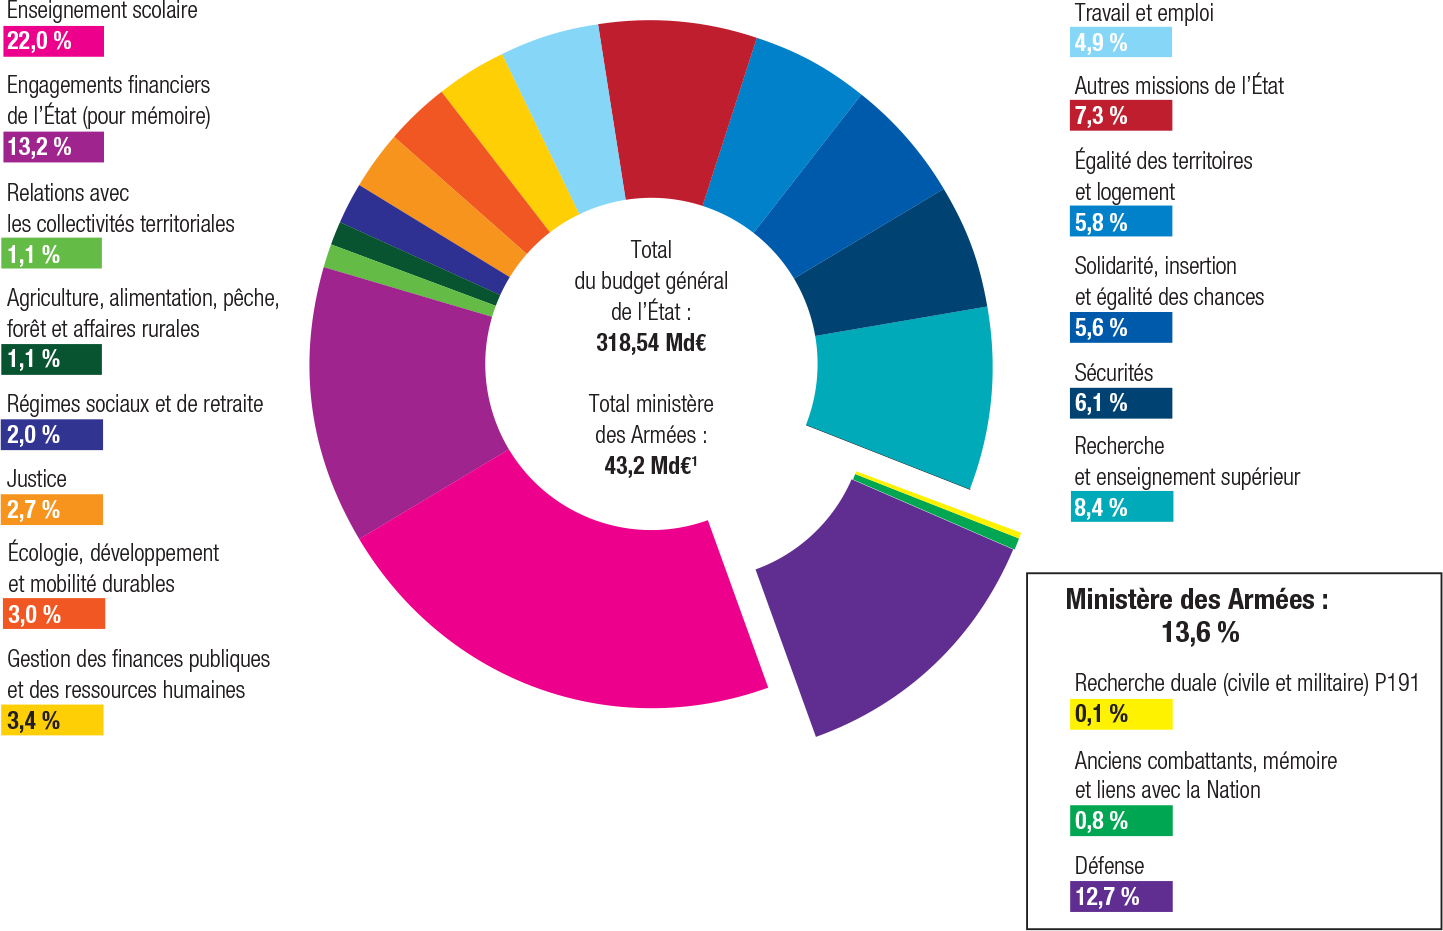
\includegraphics[width=1\textwidth]{Budget_Ministère_Défense_2017}
					\caption{Part du budget du Ministère de la Défense (pensions incluses) dans le budget général de l’État en 2017\cite{ChiffresDef2017}}%
					\label{fig:Budget_Ministère_Défense_2017}%
				\end{figure}
			\subsection{Effectifs}
				\paragraph*{}
					En 2016 le Ministère de la défense avait un effectif total de 265 458 équivalent temps plein travaillé (ETPT), composé à 77\% de militaires et 23\% de civils (voir détails sur la figure \ref{fig:Effectifs_Ministère_Défense_2016}). L'age moyen du personnel militaire était de 33,2 ans et celui du personnel civil de 47,4 ans.
				\begin{figure}[H]
					\centering%
					\resizebox{0.8\textwidth}{!}{\import{figures/}{Effectifs_Ministère_Défense_2016.tex}}%
					\caption*{\small\itshape Autres services = SCA, SSA, DGA, SGA (dont DICoD), DIRISI, SEA, SIMu, OIAS, DRM, DRSD, DGSE, DPID, DGSIC, DGRIS et EMA (partie centrale)}%
					\caption{Répartition des effectifs du Ministère de la Défense en 2016, par gestionnaire, en équivalent temps plein travaillé\cite{ChiffresDef2017}}%
					\label{fig:Effectifs_Ministère_Défense_2016}%
				\end{figure}
		\section{La Direction générale de l'Armement}
			\subsection{Historique}
				\paragraph*{}
					En 1961, le général de Gaulle crée la DMA (Délégation Ministérielle pour l'Armement) pour rationaliser la construction des matériels militaires, elle compte 6 corps d'ingénieur militaires\footnote{Les ingénieurs militaires sont des experts techniques au service de la défense}: les ingénieurs de l'aéronautique, les ingénieurs militaires des fabrications d'armement, les ingénieurs du génie maritime, les ingénieurs hydrographes de la marine, les ingénieurs des poudres et les ingénieurs militaires des télécommunications. En 1968, ils sont remplacés par un corps unique: le corps des ingénieurs de l’armement. En 1977, la DGA signifiant alors ``Délégation Générale pour l'Armement'' est créée pour remplacer la DMA.
				\paragraph*{}
					En 1995, l’arrivée de Jean-Yves Helmer au poste de délégué général pour l'armement\footnote{Jean-Yves Helmer sera a la tête de la DGA de 1996 à 2001} lancera un mouvement de regroupement et d'externalisation de la production industrielle. Regroupement d'une part par la fusion des implantations territoriales pour former 14 grands centres ainsi que la réduction du personnel qui passera de plus de 50 000 en 1995 à 9 700 en 2017. D’autre part externalisation car la DGA passe d’une structure de production d’armement à une agence de maîtrise d’ouvrages complexes. Ainsi, la DGA se séparera graduellement de ses activités industrielles.
					% \begin{itemize}
					% 	\item[1990] Le Groupement Industriel des Armements Terrestres (GIAT) de la DGA devient la société anonyme GIAT Industries (aujourd’hui Nexter System, détenu par l’État français)
					% 	\item[1991] La Direction des Constructions Navales devient une société de droit privé à capitaux publics sous le nom de DCNS (aujourd’hui Naval Group, détenu à 62,49\% par l’État français)
					% 	\item[2000] Le Service de Soutien de la Flotte (SSF) est créé pour assurer dans une structure unique la maîtrise d’ouvrage de la mise en condition opérationnelle des bâtiments de surface et des sous-marins de la Marine nationale
					% 	\item[2007] Le Service de la Maintenance Aéronautique (SMA) est transféré à l’état-major de l’armée de l’air et renommé Service Industriel Aéronautique (SIAé)
					% 	\item[2010] Le Centre d’Études de Gramat, responsable de l’évaluation des vulnérabilités des systèmes d’armes aux agressions des armes nucléaires et conventionnelles, est transféré au CEA (Commissariat à l'énergie atomique et aux énergies alternatives)
					% \end{itemize}
				\paragraph*{}
					Le 5 octobre 2009, le décret n°2009-1180\cite{DEFD0918712D} officialise le changement de nom et d'organisation de la ``Délégation Générale pour l'Armement'' qui devient dès lors ``Direction Générale de l'Armement'', toujours abrégé DGA.
			\subsection{Missions}
				\paragraph*{}
					La DGA est une direction du Ministère des Armées, elle dépend non pas du Chef d’État-Major des Armées mais directement du ministre de la Défense. Elle a de très nombreuses missions (listées dans le décret n°2009-1180\cite{DEFD0918712D}, Article 1) dont on peut extraire trois missions principales:
				\p{Équiper les forces armées}
					Maître d'ouvrage des programmes d'armement, la DGA est responsable de la conception, de l'acquisition et de l'évaluation des systèmes qui équipent les forces armées. Son action couvre toute la durée de vie de ces programmes.
				\p{Préparer l'avenir}
					Imaginer les futurs possibles, anticiper les menaces et les risques, préparer les capacités technologiques et industrielles, dans un cadre européen.
				\p{Promouvoir les exportations d'armement}
					Contribuer activement aux exportations d'armement tant sur l'aspect contrôle pour le respect des engagements internationaux de la France que sur l'aspect économique pour le développement des entreprises de défense.
			\subsection{Organisation}
				\paragraph*{}
					Depuis le 9 août 2017, Joël Barre est Délégué Général pour l'Armement (voir organigramme en Annexe \ref{sec:organigrammedga}), ce dernier, pour mener a bien les missions de la DGA, s'appuie sur différents services (dont les attributions exactes sont détaillées dans le décret n°2009-1180\cite{DEFD0918712D}), organisés la plupart du temps sous forme matricielle:
				\p{Direction du Développement International} % décret n°2009-1180\cite{DEFD0918712D}, Article 6
					La Direction du Développement International (DI) est chargée de la promotion des exportations d’armement en s’appuyant notamment sur le réseau des attachés d’armement. Elle anime et coordonne le soutien de l'État aux industriels exportateurs, en liaison étroite avec les états-majors et le réseau diplomatique.
				\p{Direction des opérations} % décret n°2009-1180\cite{DEFD0918712D}, Article 4
					La Direction des Opérations\footnote{anciennement direction des systèmes d'armes} (DO) est chargée de la conduite des programmes et opérations d'armement, et est chargée de l’exécution des travaux d'études en amont. La DO est chargée de l'acquisition des systèmes d'armes, équipements de défense, matériels et logiciels en liaison avec les états-majors, et en assurant la cohérence entre les programmes.
				\p{Direction de la Stratégie} % décret n°2009-1180\cite{DEFD0918712D}, Article 5
					La Direction de la Stratégie (DS), à Bagneux, est en charge de la stratégie pour la recherche technologique, l’industrie, et les programmes d’armement menés en coopération en s'appuyant notamment sur la MRIS (Mission pour la Recherche et l’Innovation Scientifique).
				\p{Direction des Plans, des Programmes, et du Budget} % décret n°2009-1180\cite{DEFD0918712D}, Article 8
					La Direction des Plans, des Programmes, et du Budget (DP\footnote{anciennement DPBG}) est chargée de la planification, de la programmation, de la préparation et de l'exécution du budget et assure la maîtrise financière et comptable des opérations d'armement conduites par la DGA.
				\p{Services de soutien} % décret n°2009-1180\cite{DEFD0918712D}
					Le service central de la modernisation et de la qualité (SMQ), l’inspection, le département central d’information et de communication (COMM), le service de la sécurité de défense et de l’information (SSDI), la direction des ressources humaines (DRH), la gendarmerie de l’armement (GArm).
				\p{Direction Technique} % décret n°2009-1180\cite{DEFD0918712D}, Article 7
					La Direction Technique (DT) assure les activités d’essai et d’expertise des matériels et des technologies militaires à l’aide de différents pôles de compétences. De nombreux centres d’expertise et d’essais interviennent dans le test des technologies de pointe, ces derniers sont dispersés sur toute la France (voir la figure \ref{fig:Carte_centres_expertise_et_essais_DGA}).
					\begin{figure}[H]
						\centering
						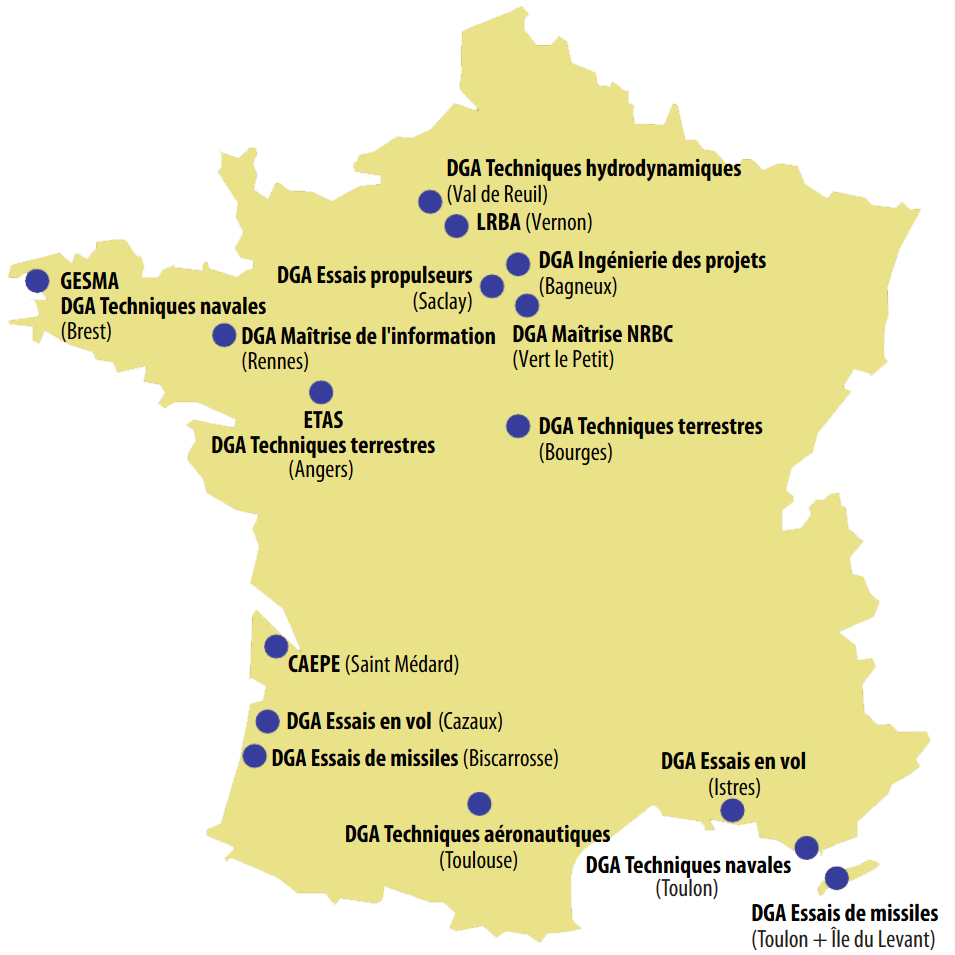
\includegraphics[width=0.9\textwidth]{Carte_centres_expertise_et_essais_DGA}
						\caption{Carte des centres d’expertise et d’essais de la DGA\cite{OptroDefDGA}}
						\label{fig:Carte_centres_expertise_et_essais_DGA}
					\end{figure}
			\subsection{Effectifs et budget}
				\paragraph*{}
					En 2017 la DGA a un effectif de 9 700 personnes dont plus de 51\% d'ingénieurs et cadres\cite{PresentationDGA}. Bien que membre à part entière du ministère de la Défense, la DGA se distingue par une forte proportion de civils au sein de son personnel, 55,7\% pour la DGA contre une moyenne de 22,9\% pour le Ministère de la Défense dans son ensemble en 2015\cite{ChiffresDef2016}, mais aussi par la quasi-absence de sous-officiers, aucun pour la GDA contre une moyenne de 44,9\% pour le Ministère de la Défense dans son ensemble en 2016\cite{ChiffresDef2017}.
				\paragraph*{}
					Le budget de la DGA n'est pas public, mais représente une part conséquente du budget du Ministère de la défense pour pouvoir maintenir, en 2017, 80 programmes d'armement et maintenir sa position de premier investisseur public de France, avec près de 11 milliards d'euros de commandes passées pour la seule année 2017. De plus la DGA maintient une présence internationale dans 20 pays, y compris auprès de l'OTAN et de l'Union européenne\cite{PresentationDGA}.
	\chapter{TODO}
		\section{TODO}
			\subsection{TODO}
				\subsubsection{TODO}
					\p{TODO}
						TODO
						\begin{upmcaution}
							This is an example of a caution message. This text must be rendered with enough height (usually 2 lines of text) to avoid intersection between the caution icon and the box frame.
						\end{upmcaution}
						\begin{upminfo}
							This is an example of an information message. This text must be rendered with enough height (usually 2 lines of text) to avoid intersection between the caution icon and the box frame.
						\end{upminfo}
						\begin{upmquestion}
							This is an example of a question message. This text must be rendered with enough height (usually 2 lines of text) to avoid intersection between the caution icon and the box frame.
						\end{upmquestion}
	% Bibliographie
	\nocite{*}
	\bibliographystyle{ieeetr-fr}
	\bibliography{references}
	\chaptertoc{Annexes}\markboth{ANNEXES}{}
		\setcounter{section}{0}
		\renewcommand{\thesection}{\Alph{section}}
		\renewcommand{\theHsection}{appendixsection.\Alph{section}}
		\section{Organigramme de la DGA}\label{sec:organigrammedga}
			\begin{figure}[H]
				\centering
				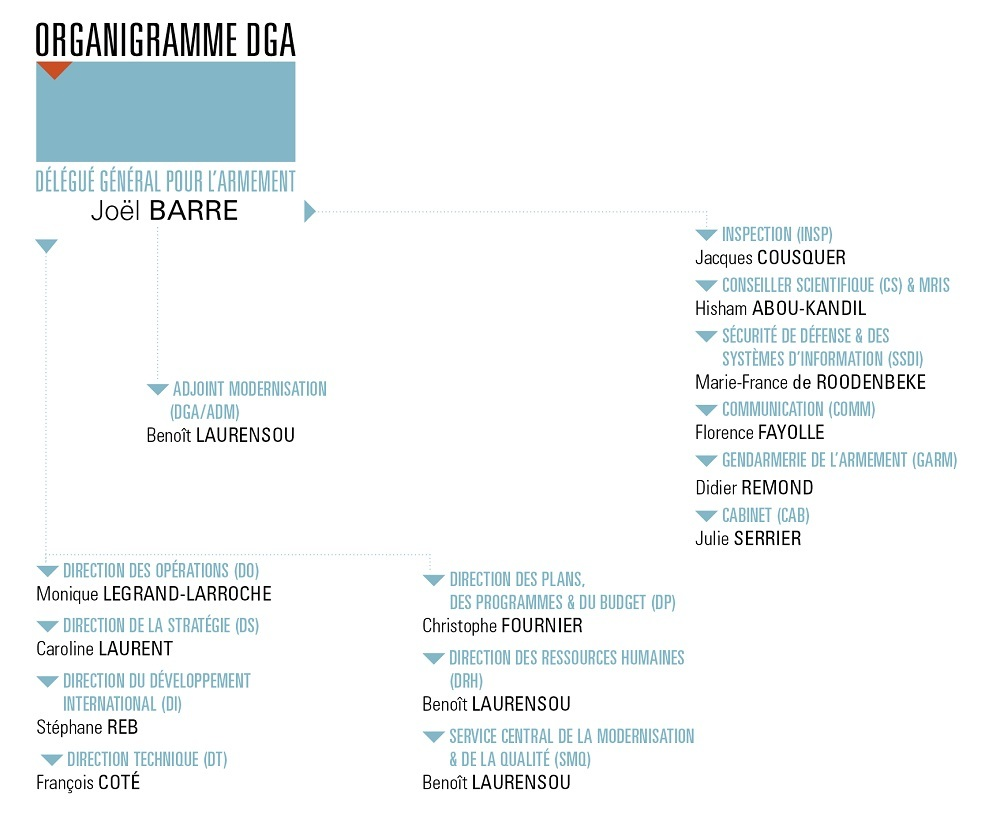
\includegraphics[width=\textwidth]{Organigramme_DGA}
				\caption{Organigramme de la DGA\cite{OrganigrammeDGA}}
				\label{fig:Organigramme_DGA}
			\end{figure}
\end{document}
